\section{Manutenzione}

\subsection{Aggiunta e aggiornamento librerie}
L'elenco delle librerie è presente nella cartella di root del programma nel file "\textit{requirements.txt}".

\begin{figure}[H]
    \centering
    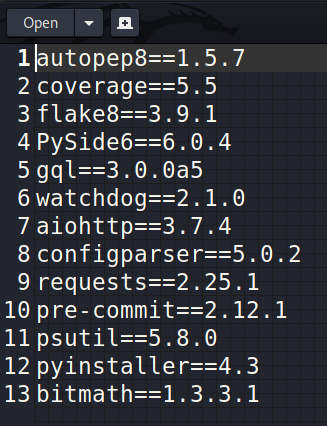
\includegraphics[scale = 0.5]{components/img/requirements.png}
    \caption{Struttura file contenente le librerie}
    \label{fig:Struttura file contentente le librerie}
\end{figure}
Per poter installare una nuova libreria il procedimento è semplice:
\begin{itemize}
	\item Aprire il file "\textit{requirements.txt}";
	\item Posizionarsi a fine file;
	\item Aggiungere una nuova riga;
	\item Aggiungere la nuova libreria.
\end{itemize}
La sintassi per l'aggiunta della libreria è la seguente:
\newline{} \centerline{\textbf{nome\_libreria==numero\_versione}}\newline{} 

\subsection{}